\chapter{Op Amps}

\section{MCP 3008}

The MCP 3008 is an 8 channel, 10 bit A/D converter that is bus addressable.  Communication is through a SPI bus.  Our Raspberry Pi has hardware support\footnote{If you had a controller that didn't have hardware support you would have to implement it in software, which is very slow and called bit banging.  I have included a bit banging code for your reference in the code part of lab 3.}.  There are four code sequences I have provided:
\begin{enumerate}
\item mcp3008bitbang.py - slow software SPI bus.  Don't use, this is only for reference if you don't have a system with hardware support.
\item mcp3008hw.py - fast hardware SPI bus.  outputs values on command line to 3 decimal places.  Good for getting precise values, but bad for lots of values.
\item mcp3008plot.py - hardware SPI bus that plots the results on a graph.  Tends to be slow because it has to sample and plot.
\item mcp3008plot-thread.py - multi-threaded hardware SPI bus that plots the result on a graph.  Yes I was having fun...  This has three threads, one that reads, one that outputs a square wave, and one that plots.  Syntax for the plot commands follows MatLab standards.  Fast and oh so much fun.
\end{enumerate}
These, of course, require library support so we have written an install shell script.  You will need to navigate to where it is located, change its permissions so it is executable, then run it.  From a terminal window type:

\CommandLine{cd ~/code/labs/labs}

\CommandLine{chmod 755 \url{install_python_libs.sh}}

\CommandLine{\url{./install_python_libs.sh}}

The mcp3008 has an analog power reference(Vref) and ground and a digital power (Vdd) and ground.  Vdd must always be connected to 3v3 (3.3V) and its ground (pin 9) to ground.  Vref and analog ground define the voltage range to compare.  Often this is the same, but it doesn't have to be.  For instance, connecting to 5v gives a bigger swing.  Remember that the chip only has 10 bits of precistion (just over 1000 divisions) and thus the precision is:
$$
\frac{Vref-Agnd}{2^{10}}
$$
Thus the larger the reference swing, the less precise the measurement.  If you want to measure something small, you should have a small reference!  The basic hookup is thus

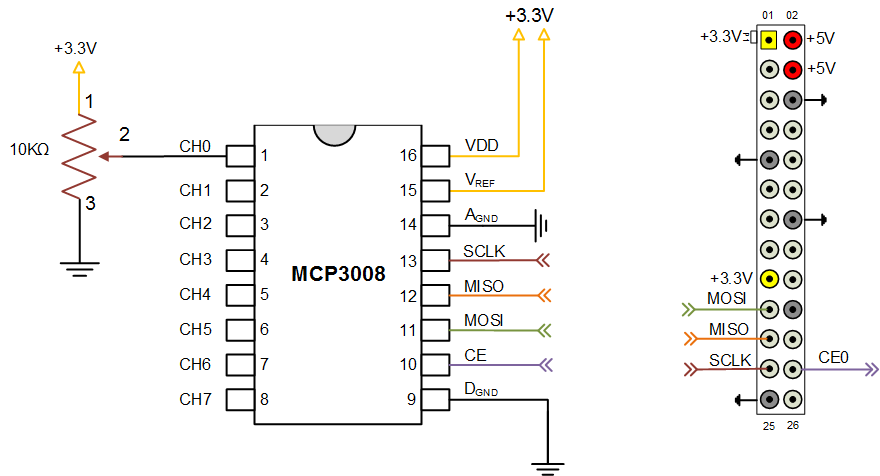
\includegraphics[width=0.8\textwidth]{../images/mcp3008_circuit.png}

Note the voltage divider on the left is only for testing and does not need to be done each time.  You will build the divider the first time to test your code and setup.  The 8 pins on the left are now available for measuring your circuit.

\section{Follower}

We will be using a general purpose 741 Op Amp.  We will connect the positive rail to 3v3 and the negative rail to ground.  Hook the output to the negative input and the signal to follow goes on the positive input.  The pinout of the 741 is:

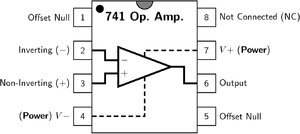
\includegraphics[width=0.4\textwidth]{../images/300px-Generic_741_pinout_top.png}


\section{Inverting Amplifier}

Note we thus can't get negative voltages, but we have no choice since we don't have a negative voltage.  We can make a new reference ground by a voltage divider between 5v and ground with identical resistors (say around 1k each) or a potentiometer around a few k\footnote{hook 5v to one outer pin and ground to the other, the center tap is the reference}, so the center will be 2v5.  Hook this to the positive input, and the rails should be connected to 5v and ground.  Hook the Vref on the MCP3008 to 5v.  Now make another potentiometer voltage divider, this time running from the op amp's output to gpio 4, with the central tap going to the op amp's negative (inverting) input.



